Here, we describe how we fitted the model for the resource-rational objective function  and how we computed next-word predictions $p(\nextWord|\representation)$.
Our fitting method is based on successful recent approaches to formally related models in various domains of machine learning  \citep{lei2016rationalizing,hahn_modeling_2016,miao2016language, seo2017neural, yu2017learning, hansen2019neural, lee2019learning}.
These are general techniques that may also be applicable to other rational and resource-rational models in cognition.

Our Python code for optimizing retention probabilities and calculating model surprisal is available at \url{https://gitlab.com/m-hahn/resource-rational-surprisal/-/tree/main/model}.






\begin{figure}
    \centering
        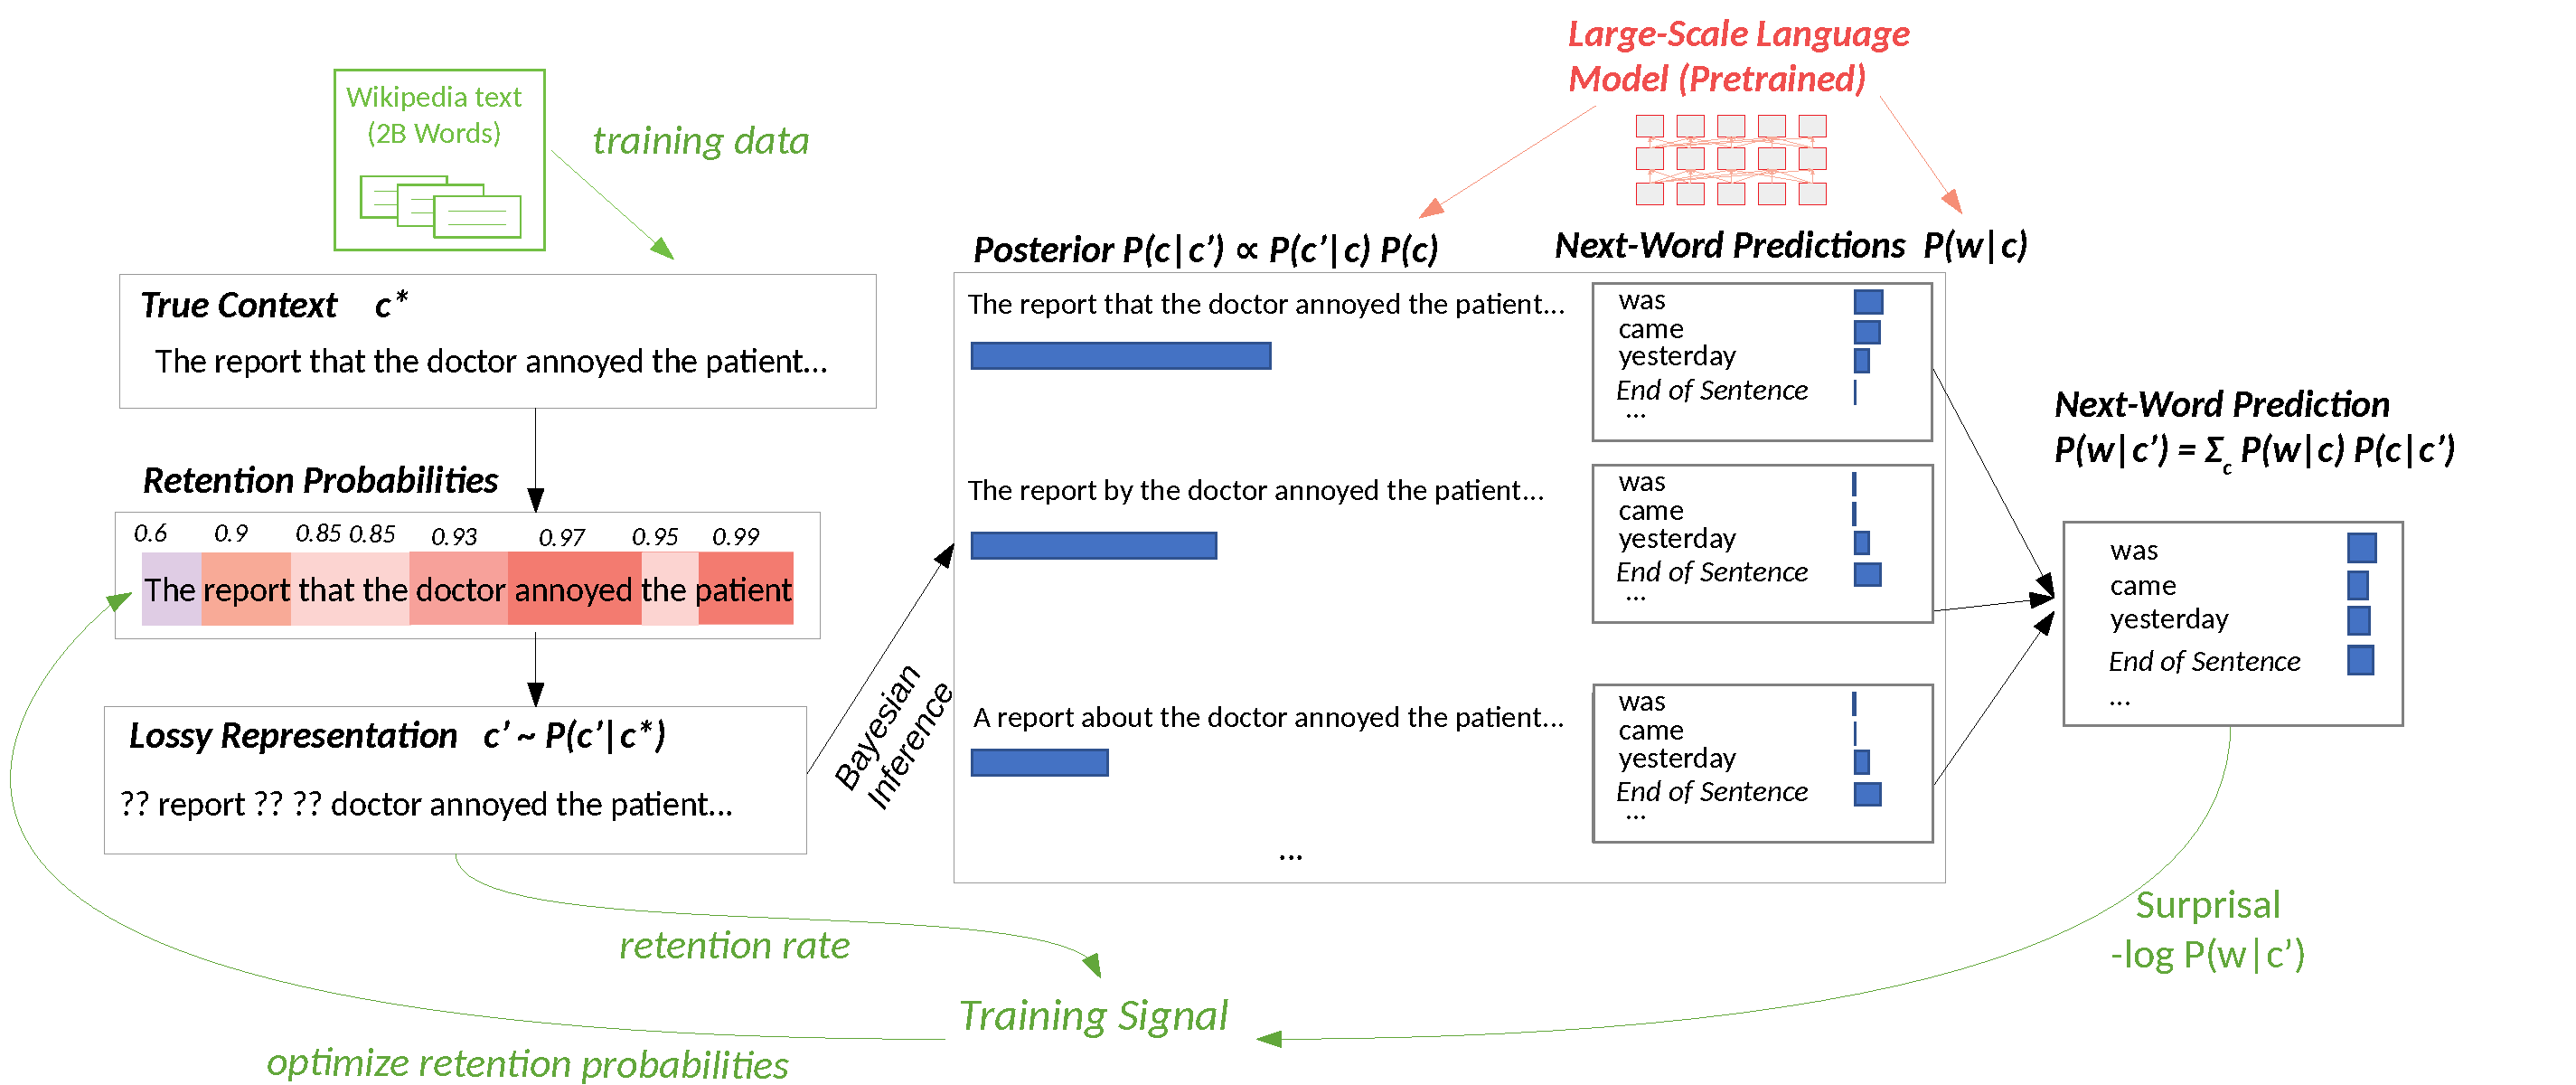
\includegraphics[width=0.9\textwidth]{figures/architecture-joint-new-si.pdf}

    
	\caption{Implementation, including fitting procedure (green) and inference (red). Compare Figure 2 in the main paper. The model is fitted on text from the English Wikipedia, unrelated to the center embedding stimuli of interest. The training signal consists of the model surprisal incurred on the next word, and a constraint on the number of retained words; the retention probabilities are optimized to minimize surprisal under an upper bound on the average number of retained words. When computing model predictions (red), both the prior $P(c)$ and the next-word probabilities $P(w|c)$ are computed using a large-scale pretrained language model, GPT-2.}
    \label{fig:model-training-viz}
\end{figure}



\subsection{Formal Description and Parameterization of Model}
Before describing the method used for fitting the model, we revisit the definition of the model formally, and describe how it is parameterized in our implementation.

\paragraph{Representation of Context}
The model operates on contexts $\contextInput = \contextInput_{1} \dots \contextInput_N$.
For the purpose of computational implementation, we set a bound $N=20$ on the maximum size of the context, long enough to accommodate all prefixes in the stimuli.
The model is fitted on continuous text, across sentence boundaries.

In line with standard practice in natural language processing, punctuation symbols (e.g., ``.'') are treated as individual tokens.
The model is constrained to never forget periods or other kinds of punctuation, which helps maintain information about sentence boundaries.
However, we remove commas from the text data as they might provide confounding cues to hierarchical structure.

For implementation reasons, neural network models have a bounded vocabulary of the most common words, and low frequency words are represented by an out-of-vocabulary (OOV) token.
We selected the 50,000 most common words in the training set for the vocabulary.
We constrained the model to never erase the OOV token, in order to prevent situations where the posterior assigns high probability to inputs where erased words have been reconstructed as OOV -- such inputs may not have a well-defined syntactic structure, which could make next-word surprisals meaningless.



\paragraph{Likelihood}
The model is defined by a family of retention probabilities $\theta = \{q_{w, i} : i,w\}$ where $w$ ranges over words and $i=1,\dots, N$.
Then $\representation=\representation_1\dots \representation_N$ is given by determining every $\representation_i$ independently as
\begin{equation}
	\representation_i = \begin{cases}\contextInput_i & \text{with probability } q_{\contextInput_i,N-i} \\
		\textsc{erased} & \text{otherwise}
	\end{cases}
\end{equation}
Thus, given an input $\contextInput = \contextInput_1\dots \contextInput_N$, $\memoryModel$ gives rise to a likelihood $p_\memoryModel(\representation|\contextInput)$.


\paragraph{Parameterizing the Model $p_\memoryModel(\representation|\contextInput)$}
The key to parameterizing the model is to parameterize the retention probabilities $q_{w,d}$.
For this, we draw on standard machine learning techniques from Natural Language Processing.
Word identity is encoded through word embeddings~\citep{DBLP:series/synthesis/2017Goldberg}, i.e., assigning a vector to each word in the vocabulary.
Relative positions are encoded though positional embeddings, i.e., assigning a vector to each of the integers $i = 1, \dots, N$  \citep{vaswani2017attention}.
The machine learning literature has identified several effective methods for combining pairs of embeddings into scalars.
We found that a deep bi-affine model \citep{Dozat2017DeepBA} yielded the best value for the resource-rational objective function.
We made this choice purely on the basis of the achieved objective function, without considering model predictions on recursive structure.
The deep bi-affine model is given by
\begin{equation}\label{eq:biaffine}
q_{w,d} := \sigma\left(  v p_i + w \cdot \operatorname{ReLU}(A x_i) + p_i^T \cdot B \cdot \text{ReLU}(C x_i)\right)
\end{equation}
where $x_i \in \mathbb{R}^{d_{word}}$ is the word embedding, $p_i \in \mathbb{R}^{d_{pos}}$ the positional embedding, $v \in \mathbb{R}^{d_{pos}}, w \in \mathbb{R}^{d_{hidden}}$ are parameter vectors, and
$A \in \mathbb{R}^{d_{hidden} \times d_{word}}$,
$B \in \mathbb{R}^{d_{pos} \times d_{hidden}}$,
$C \in \mathbb{R}^{d_{hidden} \times d_{word}}$ are parameter matrices.
$\sigma$ is the sigmoid or inverse-logit function.
We chose the dimensionalities to be $d_{word} = 1024$, $d_{pos} = 256$, $d_{hidden} = 500$ to optimize the objective function.
We initialize the word embeddings from those of the pretrained inference network $q_\theta(\nextWord|\representation)$ (see below, Section~\ref{sec:optimization-method}).
$B$ is initialized at zero \citep{Dozat2017DeepBA}.
The other parameters are initialized randomly using the defaults of the PyTorch library \citep{Paszke2019PyTorchAI}.

\subsection{Objective Function}\label{sec:variational}
Recall the objective function for the retention probabilities $\theta = \{q_{w, i} : i,w\}$:
\begin{equation}\label{eq:objective-si}
	\min_\theta \mathbb{E}_{c^*w} \mathbb{E}_{\representation \sim p_\theta(\representation|\contextInput^*)} \left[- \log p(w|\representation)\right]
\end{equation}
where $c^* w$ are contexts in the corpus together with the next words,
subject to the constraint that an average of at most $\deletionRate$ words are retained on average across contexts:
\begin{equation}\label{eq:objective-erasure-si}
	\mathbb{E}_{c^*} \mathbb{E}_{\representation \sim p(\representation|\contextInput^*)} \left[\#\{i : \representation_i \neq \text{\textsc{erased}}\}\right] \leq \deletionRate \in \mathbb{R}_+.
\end{equation}
Here, the retention rate $\deletionRate$ is a parameter, varied from 1 to 19 in the model simulations (see Figure~\ref{fig:model-surprisal})
This problem can be solved efficiently by combining neural variational inference  \citep{mnih2014neural, kingma2014auto} with Lagrangian duality \citep{Boyd2006ConvexO}.
Neural variational inference 
combines the problems of optimizing $\memoryModel$ and estimating $p(\nextWord|\representation)$ (which depends on the posterior $p(\contextInput|\representation)$, and thus ultimately on $\memoryModel$) into a single optimization problem, using auxiliary neural networks that provide learned representations of the posterior and that are optimized simultaneously with $\memoryModel$.
Thus, we expresses $p(\nextWord|\representation)$ using a powerful function approximator $q_\psi(\nextWord|\representation)$, with parameters $\psi$ chosen to minimize the KL-Divergence between the approximator and the true predictive distribution.
Such a network is referred to as an \textit{inference network} \citep{mnih2014neural, kingma2014auto}.
Using this method, we rewrite (\ref{eq:objective-si}) as
\begin{equation}\label{eq:objective-with-amortized}
	\min_{\theta, \psi} \mathbb{E}_{\contextInput^*\nextWord} \mathbb{E}_{\representation \sim p_\theta(\representation|\contextInput^*)} \left[- \log q_\psi(w|\representation)\right]
\end{equation}
Using Gibbs' Inequality \citep{Cover2005ElementsOI}, one can prove that this problem is equivalent to (\ref{eq:objective-si}), provided that the family of approximators is sufficiently expressive (such as a family of neural networks).
Finally, to efficiently take the constraint~(\ref{eq:objective-erasure-si}) into account, we draw on Lagrangian duality.\footnote{We established the validity of the Lagrangian dual objective as follows.
Note that, a priori, for nonconvex problems such as the one we are considering, the mini-max problem (\ref{eq:variational-lagrangian}) need not be equivalent to the original problem, as the solution $(\theta,\psi)$ of the mini-max problem need not satisfy the constraint (\ref{eq:objective-erasure-si}).
However, we empirically observe that the parameters $\theta$ obtained by solving (\ref{eq:variational-lagrangian}) do satisfy the constraint.
In this case, the optimal solution for (\ref{eq:variational-lagrangian}) has $\kappa = 0$.
We then note $\mathcal{L}_1(\theta, \psi, 0) = (\ref{eq:objective-si})$, establishing the equivalence of the dual problem with the original problem.
}
We thus obtain the following optimization problem:
\begin{equation}\label{eq:variational-lagrangian}
	\min_{\kappa \leq 0} \max_{\theta, \psi}  \mathcal{L}_1(\theta, \psi, \kappa)
\end{equation}
where
\begin{equation}\label{eq:lagrangian}
	\mathcal{L}_1(\theta, \psi, \kappa) := \mathop{\mathbb{E}}_\contextInput \mathop{\mathbb{E}}_{\representation \sim p_\memoryModel(\representation|\contextInput)} \left[ \log q_\psi(w|\representation) + \kappa \cdot \left[\#\{i : \representation_i \neq \text{\textsc{erased}}\}\right] - \deletionRate\right]
\end{equation}
This objective function is amenable to standard optimization methods combining neural network parameterizations of $q_\psi(\nextWord|\representation)$ with gradient descent, as we describe in the following sections.


We use the same procedure to simultaneously also create a second inference network $q_\varphi(\contextInput|\representation)$ for the posterior $p(\contextInput|\representation)$, which we use as a proposal distribution when estimating surprisal~(see Section \ref{sec:importance}).
To achieve this, we maximize
\begin{equation}\label{sec:reconstruction-objective}
	\mathcal{L}_2(\varphi) := \mathop{\mathbb{E}}_\contextInput \mathop{\mathbb{E}}_{\representation \sim p_\memoryModel(\representation|\contextInput)} \log q_\varphi(\contextInput|\representation)
\end{equation}
This minimizes the KL divergence between $q_\varphi(\contextInput|\representation)$ and the true posterior $p(\contextInput|\representation)$, averaged over contexts $\contextInput$ and representations $\representation$.



\paragraph{Parameterizing the Inference Networks}
As described above, the model has two inference networks, one ($q_\psi(\contextInput|\representation)$) modeling recovery of the true context $\contextInput$ from $\representation$, and one ($q_\psi(\nextWord|\representation)$) modeling prediction of the nect word $\nextWord$ from $\representation$.
The parameterization for the inference networks follows standard sequence modeling techniques from Natural Language Processing; the precise numerical parameters were identified to optimize the numerical value of (\ref{eq:variational-lagrangian}) without considering model predictions on recursive structure.
We parameterize the prediction model $q_\psi(\nextWord|\representation)$ as a standard LSTM language model \citep{DBLP:journals/neco/HochreiterS97} with 1024 hidden units and 2 layers.
We parameterize the reconstruction model $q_\psi(\contextInput|\representation)$ using a standard sequence-to-sequence LSTM network \citep{Sutskever2014SequenceTS, Luong2015EffectiveAT}, which transduces the input $\representation = y_1 \dots y_N$ into a probabibility distribution over output sequences $\contextInput = x_1 \dots x_N$.


\subsection{Optimization Method}\label{sec:optimization-method}

Here, we describe how we solve the variational formulation~(\ref{eq:variational-lagrangian}) of the resource-rational objective function.
All choices were made to optimize the numerical value of (\ref{eq:variational-lagrangian}), without yet considering model behavior on the sentences considered in this study.


We solve~(\ref{eq:variational-lagrangian}) using stochastic gradient descent (SGD) combining ordinary backpropagation with the REINFORCE estimator \citep{Williams1992SimpleSG}, a scheme commonly used for problems similar to ours \citep{lei2016rationalizing,hahn_modeling_2016,miao2016language, seo2017neural, yu2017learning, hansen2019neural, lee2019learning}.
This leads to the following expressions for the gradients (the first line uses the REINFORCE or policy-gradient theorem, \citep{Williams1992SimpleSG}):
\begin{align}\label{eq:variational-lagrangian-gradients}
	\partial_\theta \mathcal{L}_1(\theta, \psi, \kappa) &= \mathop{\mathbb{E}}_\contextInput \mathop{\mathbb{E}}_{\representation \sim p_\memoryModel(\representation|\contextInput)} \left[ \left( \partial_\theta \log p_\memoryModel(\representation|\contextInput) \right) \cdot \log q_\psi(\nextWord|\representation) + \kappa \sum_{i=1}^N \partial_\theta q_{\contextInput_i, N-i} \right]\\
	\partial_\kappa \mathcal{L}_1(\theta, \psi, \kappa) &=\mathop{\mathbb{E}}_\contextInput \mathop{\mathbb{E}}_{\representation \sim p_\memoryModel(\representation|\contextInput)}\left[\left[{\#\{i : \representation_i=\text{\textsc{erased}}\}}\right] - \deletionRate\right] \\
	\partial_\psi \mathcal{L}_1(\theta, \psi, \kappa) &=\mathop{\mathbb{E}}_\contextInput \mathop{\mathbb{E}}_{\representation \sim p_\memoryModel(\representation|\contextInput)} \partial_\psi \log q_\psi(\nextWord|\representation)
	\\
	\partial_\phi \mathcal{L}_2(\theta, \psi, \kappa) &=\mathop{\mathbb{E}}_\contextInput \mathop{\mathbb{E}}_{\representation \sim p_\memoryModel(\representation|\contextInput)} \partial_\phi \log q_{\phi}(\contextInput|\representation) \label{eq:variational-lagrangian-gradients-4}
\end{align}
In each step, the SGD algorithm takes a sample $\contextInput=x_1\dots x_N x_{N+1}$ from the dataset and samples $\representation \sim p_\memoryModel(\representation|\contextInput)$, and then updates the parameters using the expressions inside the expectations (\ref{eq:variational-lagrangian-gradients}--\ref{eq:variational-lagrangian-gradients-4}) as (unbiased) estimates of the gradient.
In each update step, $\kappa$ is updated in direction opposite from $\psi, \theta$, and $\kappa$ was clipped to be nonpositive.

We minibatch 12 copies of each training example, independently taking one sample from $p_\memoryModel(\representation|\contextInput)$ for each copy, but did not batch different examples together. We found this to improve optimization much more than other common choices, such as taking a larger batch size with only one copy per example.
We further add a control variate \citep{Williams1992SimpleSG} that reduces variance without introducing bias.

We run SGD for 200K steps.
Empirically, we observe that the retention probabilities essentially converge, and that the objective function shows little improvement beyond this.


Learning rates and momentum are shown in Table~\ref{tab:hyperparameters}.
We found similar values of the objective function across a wide range of hyperparameters, and thus sampled different possible parameters for each model run to maximize coverage of possible hyperparameters.


We pretrain the inference networks on samples from a uniform loss model, where each word is
retrieved with 80\% probability. To eliminate potential artifacts of individual model runs, we constructed
six reconstruction posterior models $q_\varphi$ and two prediction posterior models $q_\psi$, and randomly chose
one of each every time we constructed an optimized model $\theta$. These networks were trained on the full
corpus (2.3 Billion words) with early stopping until convergence. This pretraining approach greatly
reduces computation time and speeds up model convergence. We continue training the reconstruction
network $q_\varphi(c|c')$ together with $\theta$; this is particularly important because $q_\varphi$ also serves as a proposal
distribution in surprisal computation (see Section 1.4) and thus needs to be well-adapted to the behavior
of $\theta$. However, we found that continuing training the prediction network $q_\psi(w|c')$ was computationally
costly without strong improvement of the objective function; we thus fixed it in part of the model runs to
reduce computing cost, without observing differences in the results.


\begin{table}
\begin{center}
	\begin{tabular}{ll||llll}
		Component & Parameter & Explored Range \\ \hline\hline
		Amortized Posterior & Learning Rate & 0.001, 0.01, 0.1, 0.2 \\
\hline		Memory Model & Learning Rate & 0.00002, 0.00005, 0.0001 \\
		           & Momentum & 0.5, 0.7, 0.9 \\
\hline		Dual $\kappa$ & Learning Rate & 0.01, 0.02, 0.05, 0.1, 0.2, 0.3\\
	\end{tabular}
	\end{center}
	\caption{Hyperparameters for solving the resource-rational objective function. These were selected to optimize~(\ref{eq:variational-lagrangian}), without considering model behavior on recursive structure.}
	\label{tab:hyperparameters}
\end{table}


\subsection{Posterior Inference with Importance Sampling}\label{sec:importance}

We now describe how, given optimized retention probabilities $\memoryModel$, we used importance sampling and GPT-2 to calculate model surprisal.
By the rules of probability, the surprisal of a word $\nextWord$ given a memory representation $\representation$ is given as:
\begin{equation}\label{ref:surp}
-\log p(\nextWord|\representation) =    - \log \sum_{\tilde \contextInput} P(\nextWord|{\tilde \contextInput}) p({\tilde \contextInput}|\representation)
\end{equation}
where the posterior is given by
\begin{equation}\label{eq:ref:posterior-bayes}
p({\tilde \contextInput}|\representation) = \frac{ p(\representation|{\tilde \contextInput}) P({\tilde \contextInput})}{\sum_{\tilde \contextInput} p(\representation|{\tilde \contextInput}) P({\tilde \contextInput})}
\end{equation}
Direct calculation from this expression is intractable due to the sum over all sequences in the denominator.\footnote{An alternative approach could be to directly use the inference network $q_\psi(\nextWord|\representation)$ as a stand-in for $p(\nextWord|\representation)$. However, importance sampling allows us to draw on the modeling power of GPT-2, trained on an even larger dataset than our inference network.}


A standard approach for estimating such quantities is importance sampling \citep{Hammersley1954PoorMM}, which obtains samples from a \emph{proposal distribution} from which samples can be taken easily, and reweights these to match the desired target distribution.
We use the inference network  $q_\phi(\contextInput|\representation)$ as a proposal distribution and GPT-2-Medium for the prior $P({\tilde \contextInput})$.
This leads to
\begin{equation}
p(\nextWord|\representation) \approx \frac{\sum_{i=1}^{K} w_i P(\nextWord|\contextInput^{(i)})}{\sum_{i=1}^K w_i}
\end{equation}
where $\contextInput^{(i)}$ are sampled from $p_\psi(\contextInput^{(i)}|\representation)$ and the importance weights are given as
\begin{equation}
	w_i := \frac{P(\contextInput^{(i)}) p(\representation|\contextInput^{(i)})}{p_\psi(\contextInput^{(i)}|\representation)}
\end{equation}
In our experiments, we set $K=24$ to balance computational cost with stability of estimates.

As described in the main paper, we predict human reading times from the expected model surprisal averaged over memory representations, $\mathbb{E}_{\representation \sim p(\representation|\contextInput)} \left[- \log P(\nextWord|\representation)\right]$. As the set of all possible representations is exponentially large, we computed a Monte Carlo estimate using 6 samples $\representation \sim p_\theta(\representation|\contextInput)$.
Thus, in total, model predictions are computed using $6\cdot 24 = 144$ possible contexts ${\tilde \contextInput}$ for each trial.\footnote{As our model simulations use 58 nouns paired with (in Experiment 2) 42 items and 5 conditions, it was not feasible to conduct all simulations with a larger number of samples. However, we verified that larger sample sizes led to equivalent results when subsampling a smaller set of nouns and items.}


\subsection{Model Runs}
We solved the resource-rational objective function for $\deletionRate = 1, 2, \dots, 19$.
The stochastic gradient descent optimization method described in Section~\ref{sec:optimization-method} is nondeterministic, leading to different approximate optimizers of the objective function on every run.
We created at least 4 runs for every parameter setting, and at least 10 for each setting in the range used for model predictions ($4\leq \deletionRate \leq 15$).
Model runs were run by a script that was run in parallel on multiple machines, randomly choosing configurations for which the intended number of runs had not been reached; the overall number of model runs per configuration was thus determined by compute availability and chance.
A total of 279 model runs resulted.


